%!TEX root = ../TTK4900-MHT.tex

\chapter{Radar and AIS preprocessing}\label{chapter:radar-and-ais-preprocessing}
The process from raw radar and \gls{ais} data to target tracks is made up from several processing steps. The aim of this chapter is to give the reader a basic understanding of these steps and their challenges.

\section{Radar preprocessing}\label{sec:radar_preprocessing}
Rotating maritime radars (Figure~\ref{fig:maritime_radar_antenna}) are wide and short, giving them a tall and narrow beam. A ping, transmit and receive sequence is carried out for each antenna rotation angle in the radars scan resolution. This gives reflections as signal level in spokes described by polar coordinates, rotation angle and distance. Each spoke has a width determined by the design of the antenna, primarily the width of the antenna, and a number of cells dictated by the discretization and sampling interval of each spoke. The spokes is then run through a detection algorithm, which is filtering the received signal according to detection setting. The detection algorithm is often built in to the radar system, with both fixed and user adjustable detection parameters.

When displayed on a screen in a vessel, the output from the detection step is viewed and interpreted by the operators. In an automated scenario with autonomous vessels, the next step would be to transform the detections from polar vessel body frame to for instance a Cartesian world fixed local frame. Which frame to convert to is a design choice, and can be dependent on use-case, interconnected systems and performance requirements. This transformation is strongly dependent on knowing the position and attitude of own vessel at each spoke sampling time, which is fed from the vessel's navigation system.

With all the spoke resolution cells converted to a world-fixed Cartesian coordinate system, it is desirable to remove land reflections, if any such are present. This step is dependent on highly detailed digital maps of the area in question, which are commercially available for most of the world. Since maps have both offsets and inaccuracies to some extent, a cleaner land masking can be accomplished by dilating the coastline. This is in many situations acceptable since the vessels will never be that close to shore, and any targets masked away is in a region out of interest.

The last step in the radar processing chain is to convert a point cloud into measurements, as one target will in most cases fill multiple resolution cells and therefore it does not yield good result to send all cells with detection forward as measurements. This clustering of the detections is also desirable due to the assumption that each target maximum generates one measurements. This leads to clustering algorithms that assumes that detections closely spaced are originating from the same target, and thus should be one measurement. There are many clustering algorithms available to solve this problem, some builds graphs with vertices between neighbouring detections given a neighbour criterion, some estimates the number of clusters and optimizing the detections into this number of clusters~\cite{Mahmuddin2010,Pelleg2000,Brekke2010}. When a set of detections are clustered, their respective measurement is calculated as the centroid of the polygon made from the detections, which would be weighted by their signal strength if available. These measurements are sent to the tracking module.

\subsection{Frame conversion}\label{subsec:frame_conversion}
The radar measurements is by nature in polar frame, and the target motion model is best described in a Cartesian frame. The most usual solution is to convert the radar measurements to a Cartesian frame, and to avoid biased and optimistic covariances of the converted measurements, a procedure which compensates for these errors, (\ref{eq:debiased_coordinate_conversion}) and (\ref{eq:average_true_converted_measurement_covariace}), should be used in stead of the standard conversion (\ref{eq:standard_coordinate_conversion}) and (\ref{eq:linearized_converted_measurement_covariace})~\cite{Bar-Shalom1995}.
\begin{equation}\label{eq:debiased_coordinate_conversion}
\begin{split}
\begin{bmatrix} x \\ y \end{bmatrix} &= \begin{bmatrix} r_m \cos \theta_m \\ r_m \sin \theta_m \end{bmatrix} - \mu_a \\
\mu_a & \triangleq 
\begin{bmatrix}
	E \lbrack \tilde{x}|r_m,\theta_m \rbrack \\ 
	E \lbrack \tilde{y}|r_m,\theta_m \rbrack 
\end{bmatrix} 
= 
\begin{bmatrix}
	r_m \cos \theta_m (e^{-\sigma^2_\theta}) - e^{-\sigma^2_\theta / 2} \\ 
	r_m \sin \theta_m (e^{-\sigma^2_\theta}) - e^{-\sigma^2_\theta / 2}
\end{bmatrix} 
\end{split}
\end{equation}

\begin{equation}\label{eq:average_true_converted_measurement_covariace}
\begin{split}
R_a^{11} & \triangleq r_m^2 e^{-2\sigma_\theta^2} \lbrack \cos^2\theta_m(\cosh 2\sigma_\theta^2-\cosh \sigma_\theta^2) + \sin^2\theta_m (\sinh 2\sigma_\theta^2 - \sinh \sigma_\theta^2) \rbrack \\
& + \sigma_r^2 e^{-2\sigma_\theta^2} \lbrack \cos^2 \theta_m (2\cosh 2\sigma_\theta^2 - \cosh\sigma_\theta^2) + \sin^2 \theta_m (2\sinh 2\sigma_\theta^2 - \sinh \sigma_\theta^2) \rbrack \\
R_a^{22} & \triangleq r_m^2 e^{-2\sigma_\theta^2} \lbrack \sin^2\theta_m(\cosh 2\sigma_\theta^2-\cosh \sigma_\theta^2) + \cos^2\theta_m (\sinh 2\sigma_\theta^2 - \sinh \sigma_\theta^2) \rbrack \\
& + \sigma_r^2 e^{-2\sigma_\theta^2} \lbrack \sin^2 \theta_m (2\cosh 2\sigma_\theta^2 - \cosh\sigma_\theta^2) + \cos^2 \theta_m (2\sinh 2\sigma_\theta^2 - \sinh \sigma_\theta^2) \rbrack \\
R_a^{12} & \triangleq \sin \theta_m \cos \theta_m e^{-4\sigma_\theta^2} \lbrack \sigma_r^2 + (r_m^2 + \sigma_r^2)(1-e^{\sigma_\theta^2}) \rbrack
\end{split}
\end{equation}

\begin{equation}\label{eq:standard_coordinate_conversion}
x = r_m \cos \theta_m \qquad y = r_m \sin \theta_m
\end{equation}

\begin{equation}\label{eq:linearized_converted_measurement_covariace}
\begin{split}
R_L^{11} & \triangleq r_m^2 \sigma_\theta^2 \sin^2\theta_m + \sigma_r^2 \cos^2 \theta_m \\
R_L^{22} & \triangleq r_m^2 \sigma_\theta^2 \cos^2\theta_m + \sigma_r^2 \sin^2 \theta_m \\
R_L^{12} & \triangleq (\sigma_r^2 - r_m^2 \sigma_\theta^2) \sin \theta_m \cos \theta_m \\
\end{split}
\end{equation}

\begin{equation*}
\begin{split}
r_m 			&= \text{measured range} \\
\theta_m		&= \text{measured bearing} \\
\sigma_r 		&= \text{range measurement standard deviation} \\
\sigma_\theta 	&= \text{bearing measurement standard deviation} \\
\M{R_a} 		&= \text{average true converted measurement covariance} \\
\M{R_L} 		&= \text{linearised converted measurement covariance} \\
\end{split}
\end{equation*}

\section{AIS preprocessing}~\label{sec:ais_preprocessing}
\Gls{ais} does not suffer from the association uncertainty, clutter and low accuracy like radar measurement. It does however have some issues caused by suboptimal or erroneous transmitter implementation, transmission collision caused by \gls{tdma} leading to ID (\gls{mmsi}) swaps, and delayed messages leading to out of order reception. In order to remove most of these errors, it is desirable to filter the incoming \gls{ais} messages before sending them to the tracking module.

\subsection{Out-of-order filtering}
All \gls{ais} messages are stamped with the \gls{utc} of transmission, and `frequently arrive out-of-order'~\cite{Wilthil}, illustrated in Figure~\ref{fig:out_of_order_ais}~\cite{Wilthil} (with permission).
\begin{figure}[H]
\centering
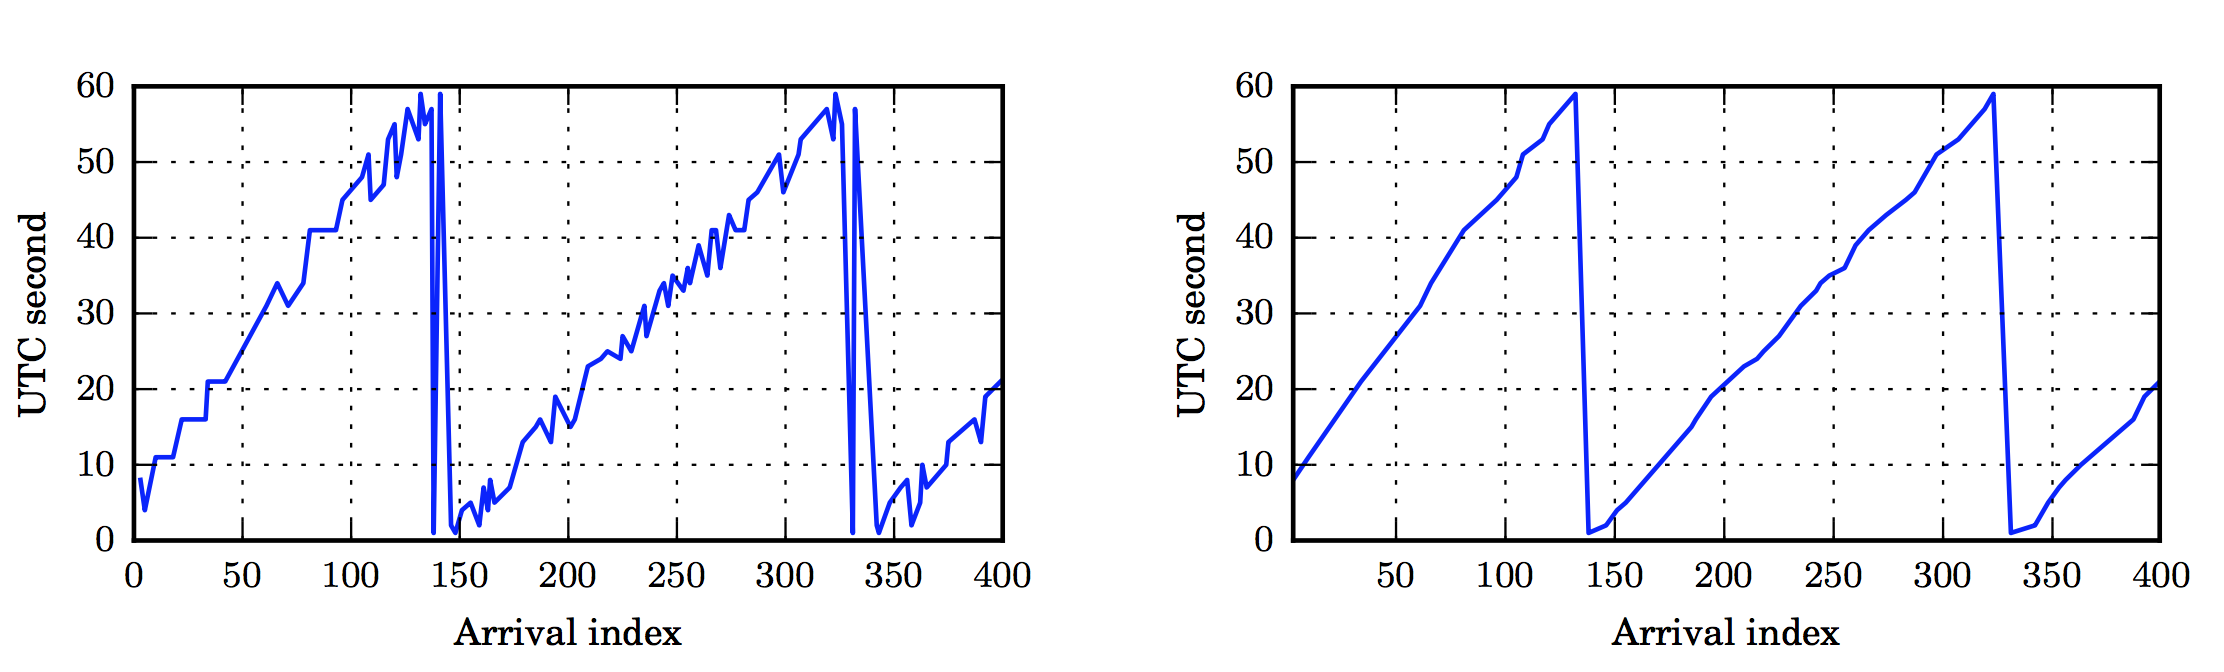
\includegraphics[width = .9\textwidth]{Figures/out_of_order_ais.png}
\caption{Unfiltered and filtered AIS arrival time}\label{fig:out_of_order_ais}
\end{figure}
One of the simplest ways of remedying this issue is to discard all messages with older timestamps that the current newest for each \gls{mmsi}. This will lead to a loss of data, which will lead to a slower AIS update period for the tracking module.

\subsection{ID swap filtering}
According to~\cite{Harati-Mokhtari2007}, 2\% of the received AIS messages in a data-mining study contained erroneous \gls{mmsi}. One of the errors were that many vessels transmitted messages with the same MMSI (11930446). This is the default MMSI on equipment from a specific manufacturer. Another example from the same study is two vessels which swapped IDs for a moment when they were passing, with a recovery after about 15 minutes. The latest example could be caused by simultaneous transmission or reflections, but the cause is not examined in the paper. Although much more rare that the out-of-order reception, ID swaps can occur and should be monitored by i.e. a logic testing \gls{ais} measurement innovations.

To remedy this issue, a simple test logic can be incorporated to check for obvious faults like sudden large position change and known default IDs. When a message and MMSI is categorized as bad, it would be held back from the tracking module. 

\subsection{Synchronization}
Since AIS messages arrive asynchronously and the tracking module is only accepting AIS updates along with radar updates, we must synchronize the incoming AIS messages. In this work, all \gls{ais} measurements are buffered from when they are received until the next radar scan.